\chapter{Data Model, API Design, and Frontend Workflows}
\thispagestyle{plain}
\section*{Introduction}
\addcontentsline{toc}{section}{Introduction}
The platform is not only a collection of services. It is also a structured data system, an API surface, and a set of user workflows. This chapter examines those three aspects together because they are tightly linked. The data model determines what can be known and queried. The API design determines how that knowledge is exposed and manipulated. The frontend workflows determine how users actually encounter and exploit the platform's capabilities.

\section{Data Modelling Principles}
The data model is shaped by four principles: service ownership, canonical identity, durable history, and contextual enrichment.

Service ownership means each service owns its own schema and tables. Canonical identity means entities that must be correlated across sources, such as indicators or CVEs, need stable identifiers or normalized values. Durable history means the platform should preserve enough information to support later reprocessing and review. Contextual enrichment means raw source data should be supplemented with fields and relationships that make operational reasoning possible.

These principles explain why the platform stores both structured relational fields and retained upstream JSON payloads, why it distinguishes entity families by service domain, and why some tables exist not to mirror an upstream feed directly but to support local intelligence work, such as notes, reports, rankings, or notification rules.

\section{Key Entity Families}
The system's stored knowledge can be grouped into several entity families.

The vulnerability family includes CVEs, EPSS records, KEV state, and AI-generated or analyst-generated relevance artefacts. The indicator family includes normalized indicators, source-level corroboration, and investigation-related artefacts. The actor family includes actors, their tools, TTP associations, ransomware groups, and victims. The orchestration family includes reports, actor-likelihood outputs, correlations, policies, and notification rules or dispatches. The identity family includes users, roles, sessions, service accounts, and audit records. The contextual family includes assets, tags, company profile, scopes, and configuration needed to interpret the rest of the knowledge base.

This grouping matters because it shows that the database is not just a passive sink of external feed data. It contains both imported intelligence and locally generated analytical state.

\section{Why the Data Model Is Hybrid}
A purely normalized relational design would make some ingestion tasks cumbersome because external sources evolve and often emit irregular payloads. A purely document-oriented design would weaken query discipline and make common filters or joins harder to reason about. The platform therefore uses a hybrid model: extract the fields needed for query, sorting, and linkage; preserve the broader upstream payload where fidelity matters.

This hybrid strategy is especially appropriate in threat-intelligence systems, where upstream schemas are heterogeneous and sometimes unstable. It allows the platform to remain query-efficient without discarding useful source context.

\section{API Design Principles}
The API layer follows five practical principles: resource orientation, typed validation, predictable status behaviour, service-local ownership, and edge composition.

Resource orientation means endpoints expose stable domain entities and workflows rather than arbitrary backend internals. Typed validation means request and response bodies are governed by Pydantic schemas. Predictable status behaviour means client code can distinguish ordinary success, validation failure, authorization failure, asynchronous acceptance, and backend error without guessing. Service-local ownership means each service exposes only its own data and behaviour. Edge composition means the frontend BFF may aggregate service responses into UI-shaped payloads without forcing backend services to become page-specific.

\section{The API Contract and Why It Matters}
The API contract is one of the most important architectural stabilizers in the platform. Backend services can evolve internally, but as long as their externally consumed contracts remain predictable, the frontend and neighbouring services can remain stable. In a multi-service system, this matters as much as database design. Poor contract discipline can make a service architecture feel more fragile than a monolith.

FastAPI and Pydantic help solve this problem by making schemas explicit and close to code. This does not remove the need for discipline, but it makes interface structure far more visible.

\section{Request Classes in the Platform}
The platform exposes several distinct classes of request.

The first class is CRUD-oriented domain requests: create, read, update, or list assets, users, rules, tags, or other managed entities. The second class is lookup requests, especially IOC lookup, where low latency is central. The third class is investigative requests, which may trigger broader enrichment or multi-source fan-out. The fourth class is synthesis requests, which either return persisted analytical outputs or trigger new analysis. The fifth class is control-plane requests, such as login, secret bootstrap, scheduler control, or health checks.

Recognizing these request classes is useful because they imply different implementation patterns. Not every endpoint should be optimized or validated the same way.

\section{Pagination, Sorting, and Filter Semantics}
A platform that ingests many entity types must avoid returning uncontrolled result sets. Pagination, sorting, and filtering are therefore not cosmetic API features. They are part of the usability and performance model. The shared helper functions and route patterns used across services indicate a deliberate attempt to keep list behaviour predictable.

This matters especially for analyst workflows. When entities such as CVEs, indicators, articles, or actors grow in number, interface usefulness depends heavily on how well the API supports ordered and filtered retrieval.

\section{Error Handling and Operator-Facing Correctness}
The platform's error design is intentionally structured. Errors are not merely log lines or ad hoc exceptions. They are translated into a consistent response shape. This is important because in a service-oriented platform, error contracts are part of correctness. The frontend and neighbouring services need to distinguish validation errors from permission failures, transient upstream issues from persistent local faults, and synchronous success from asynchronous acceptance.

The shared error-handling layer reduces accidental inconsistency in this area. That is a non-trivial engineering benefit because inconsistent error behaviour across fifteen services would quickly degrade both debugging quality and user trust.

\section{The BFF as Workflow Composer}
The BFF layer is crucial to how the frontend works. It is not merely a security proxy. It is also a workflow composer. A dashboard page, for example, often needs data from multiple backend services. It would be a mistake to force each backend service to know about the dashboard's exact payload needs. Instead, the BFF collects and reshapes the relevant data into one UI-oriented response.

This separation improves both backend cohesion and frontend simplicity. It also gives the browser one logical API surface instead of exposing every internal service contract directly.

\section{Frontend State and Interaction Model}
The frontend combines server-facing BFF routes with client-side state for authentication, permissions, and user-interface coordination. Persisted auth state makes user sessions survive refreshes. The typed client layer ensures requests remain consistent. Permission-sensitive navigation prevents users from encountering actions or pages that they are not supposed to use.

This is important from a workflow perspective because a security platform is used repeatedly under pressure. If the interface forgets state too easily, requires repeated low-value re-entry, or exposes an incoherent navigation surface, the analyst's actual working speed declines even if the backend is technically strong.

\section{Representative User Workflows}
\subsection{Login and Session Establishment}
The first workflow is identity establishment. The user logs in through the frontend, the BFF relays the request to auth, the auth service issues tokens, and the frontend stores the relevant auth state for future requests. This workflow matters because it establishes the platform's primary trust boundary.

\begin{figure}[H]
\centering
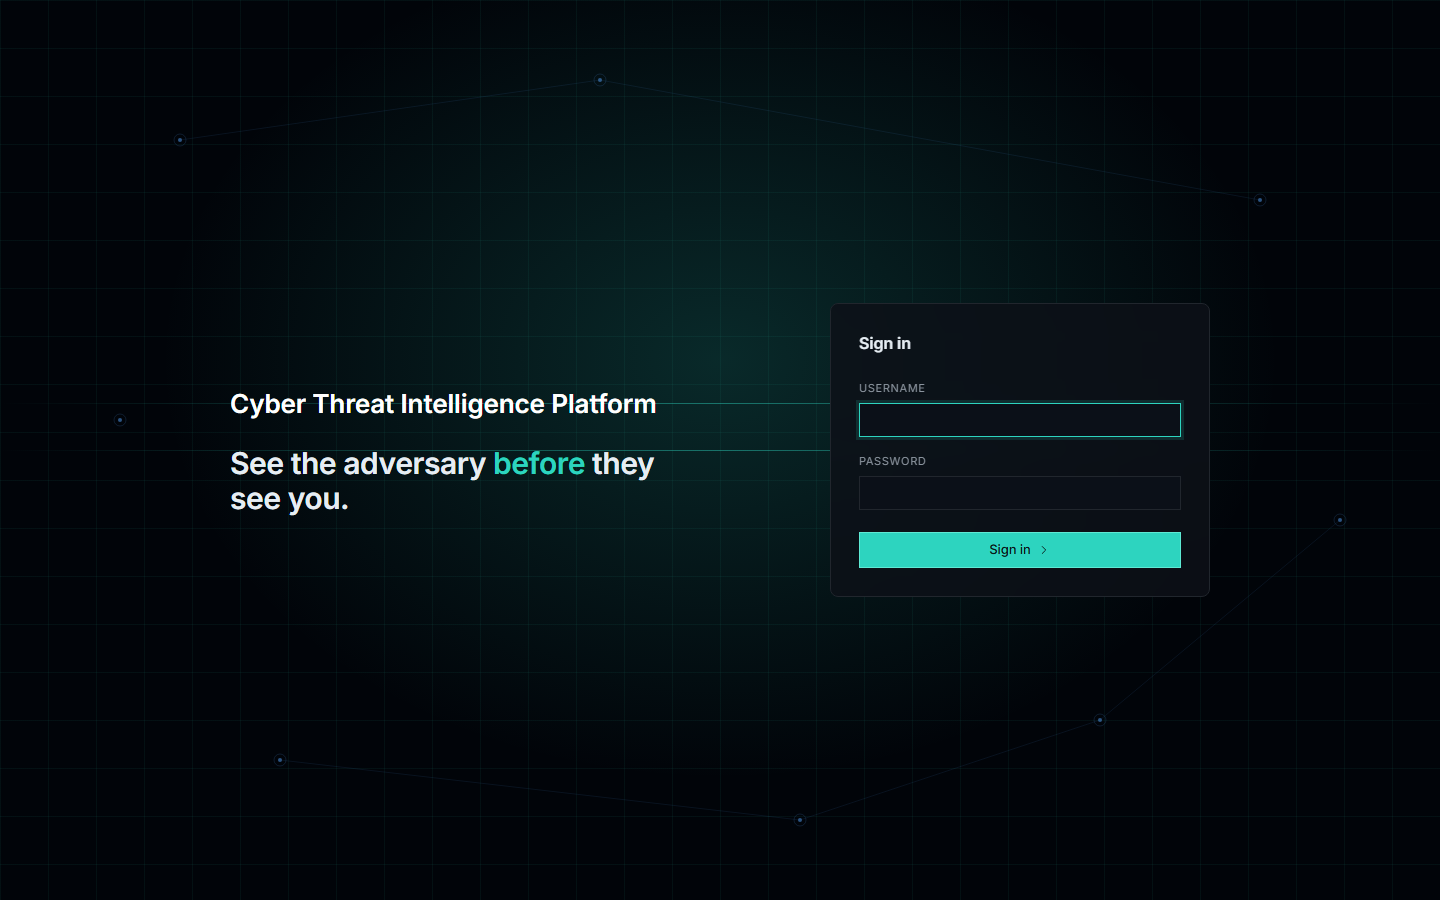
\includegraphics[width=0.82\textwidth]{images/tip/shots/01_login.png}
\caption{Login workflow entry point.}
\label{fig:login-workflow}
\end{figure}

\subsection{Dashboard Consumption}
The dashboard workflow is an aggregation workflow. The user expects a single situational view, but the backend knowledge required to produce that view comes from many services. The BFF therefore collects and reshapes the relevant data before returning it to the page.

\begin{figure}[H]
\centering
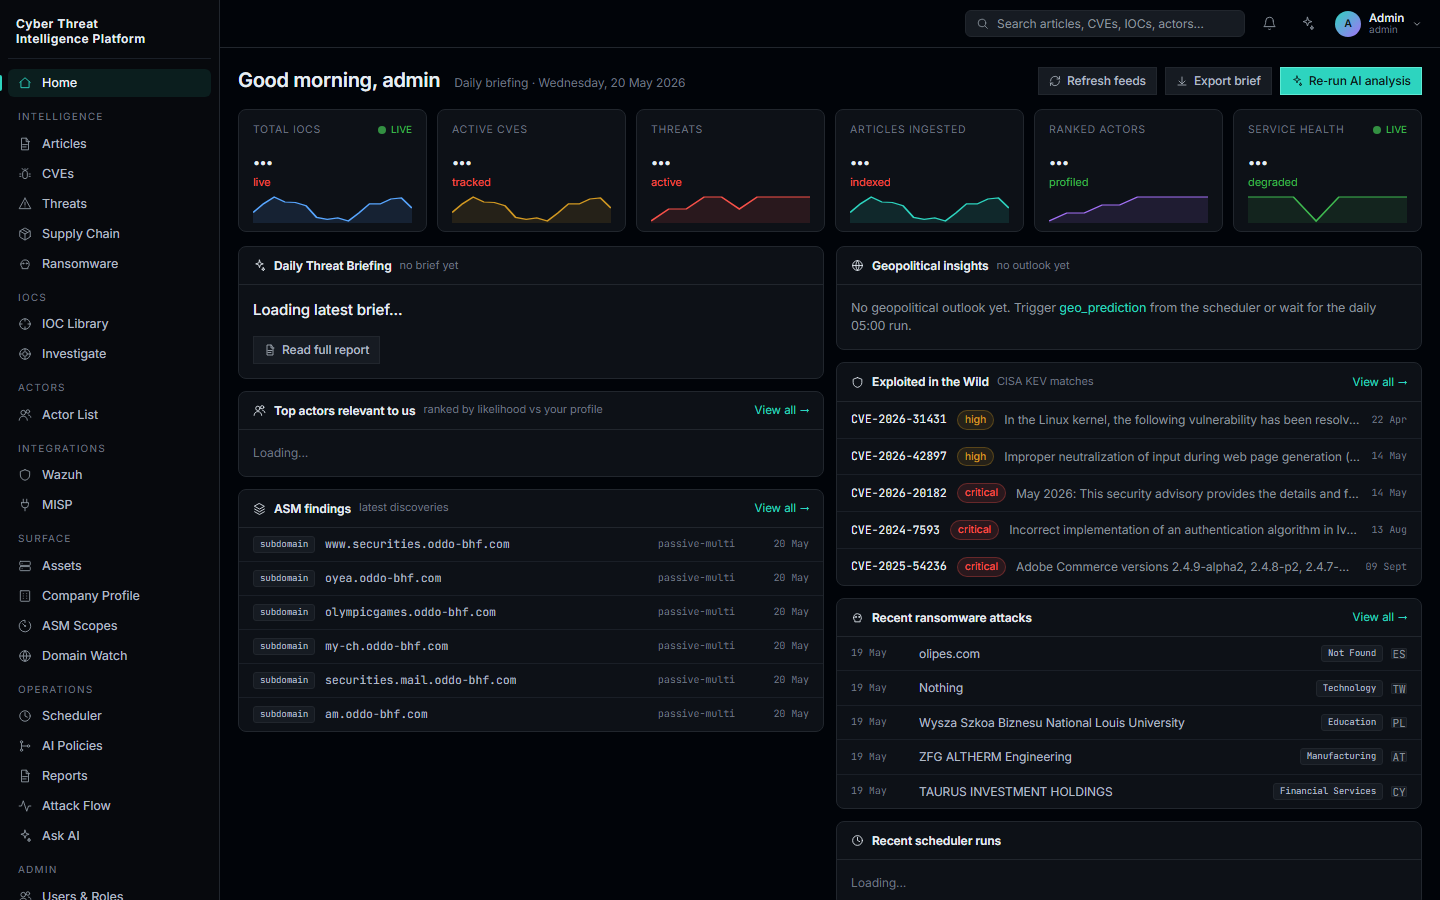
\includegraphics[width=0.9\textwidth]{images/tip/shots/02_dashboard.png}
\caption{Dashboard workflow as a composed intelligence surface.}
\label{fig:dashboard-workflow}
\end{figure}

\subsection{Article Review and Enrichment}
Article browsing and article detail workflows show how narrative reporting is converted into locally usable intelligence. The analyst can move from a list of ingested articles to deeper detail and associated insights.

\begin{figure}[H]
\centering
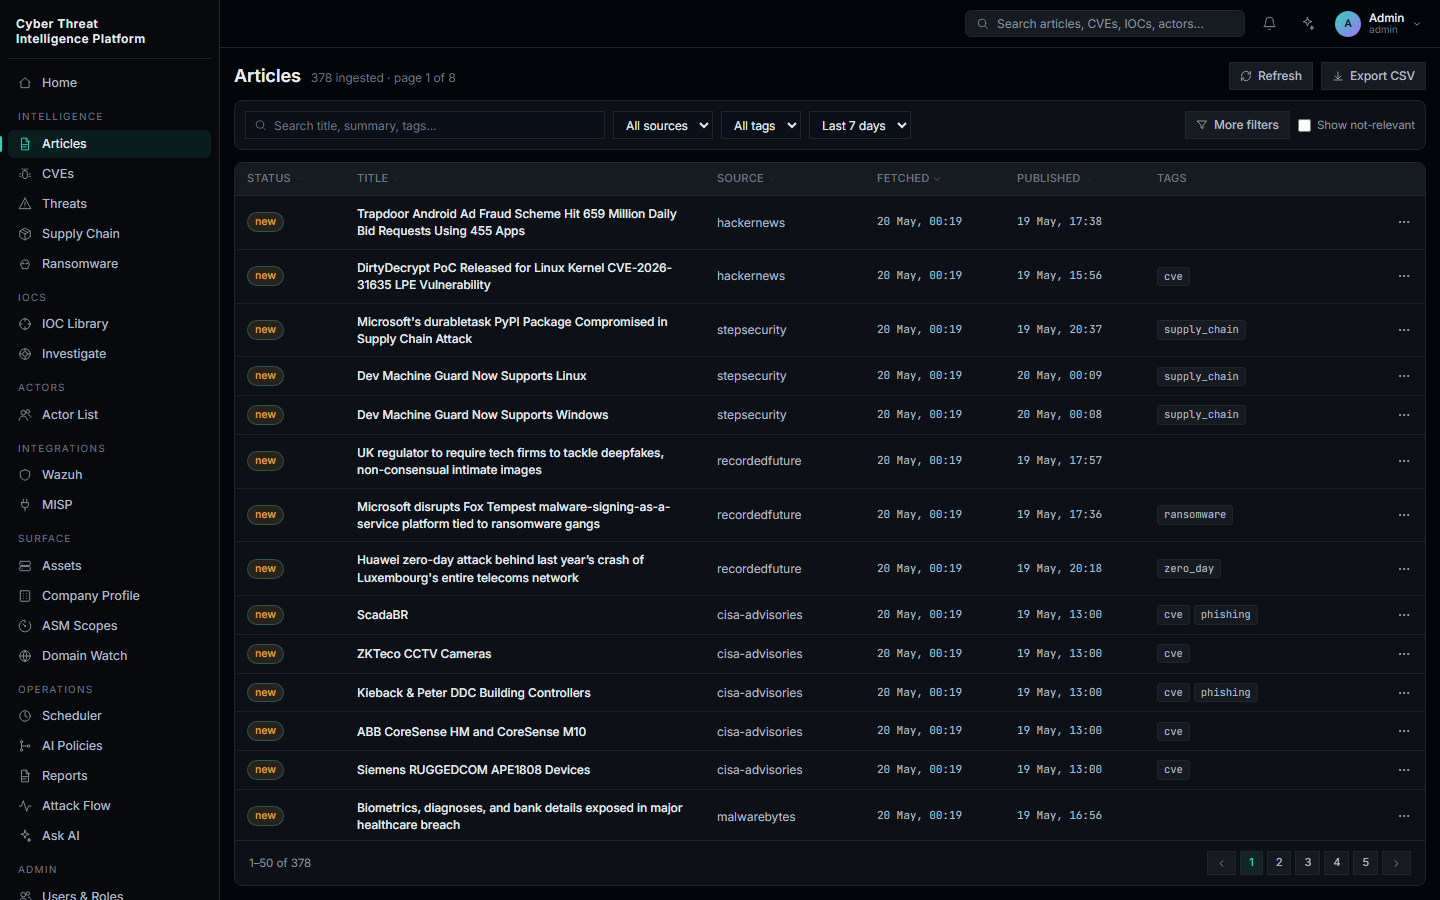
\includegraphics[width=0.9\textwidth]{images/tip/shots/03_articles_list.png}
\caption{Article-list workflow.}
\label{fig:article-list-workflow}
\end{figure}

\begin{figure}[H]
\centering
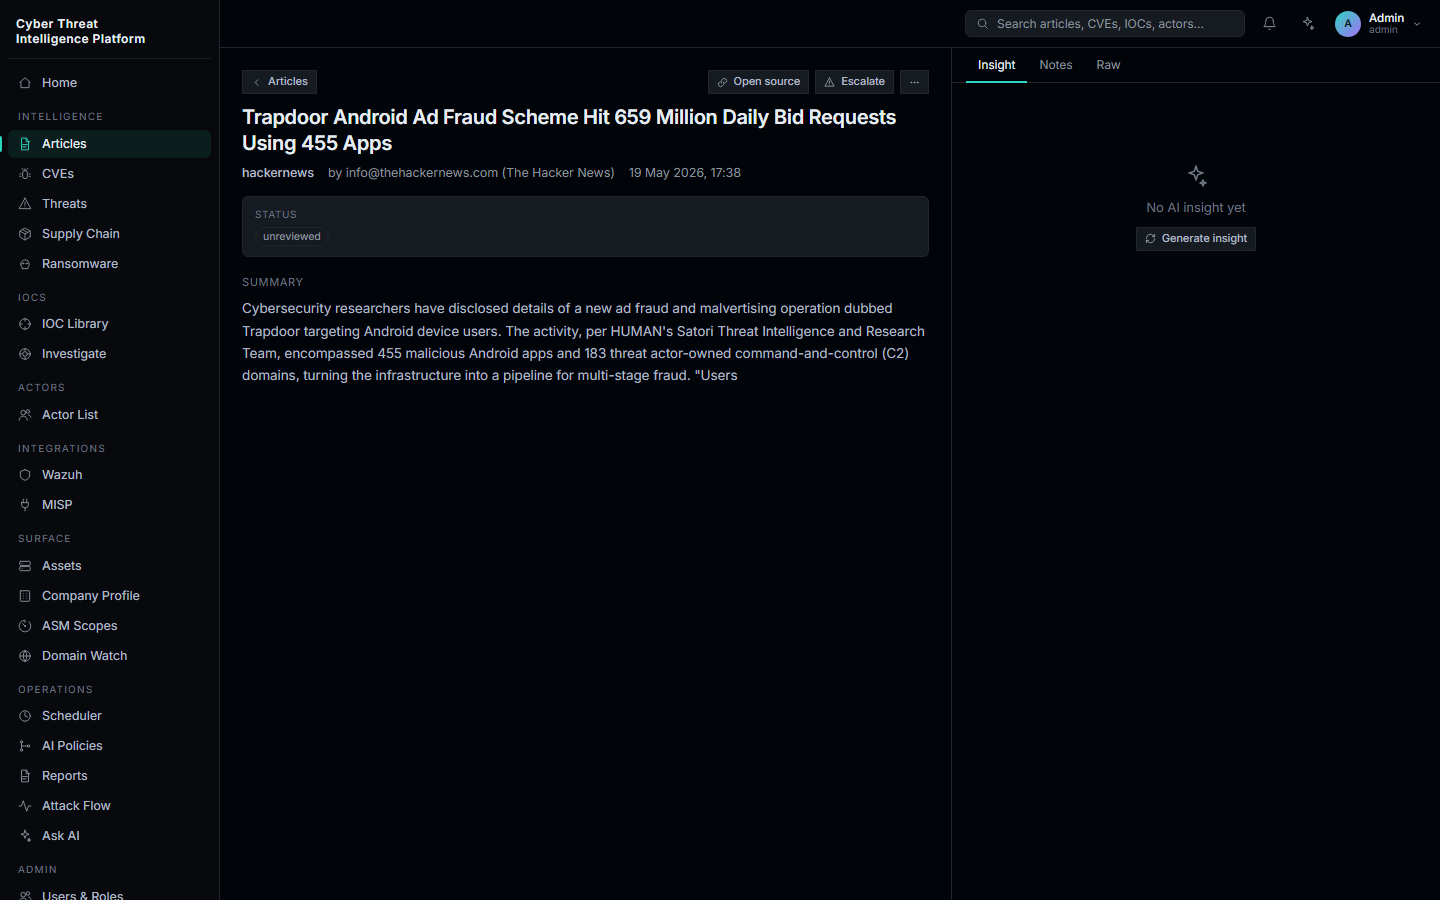
\includegraphics[width=0.9\textwidth]{images/tip/shots/04_article_detail.png}
\caption{Article-detail workflow.}
\label{fig:article-detail-workflow}
\end{figure}

\subsection{Vulnerability Prioritization Workflow}
The CVE list and CVE detail views represent one of the platform's most important analytical surfaces. They do not merely expose a feed. They provide a context in which vulnerabilities can be interpreted relative to exploitability and local relevance.

\begin{figure}[H]
\centering
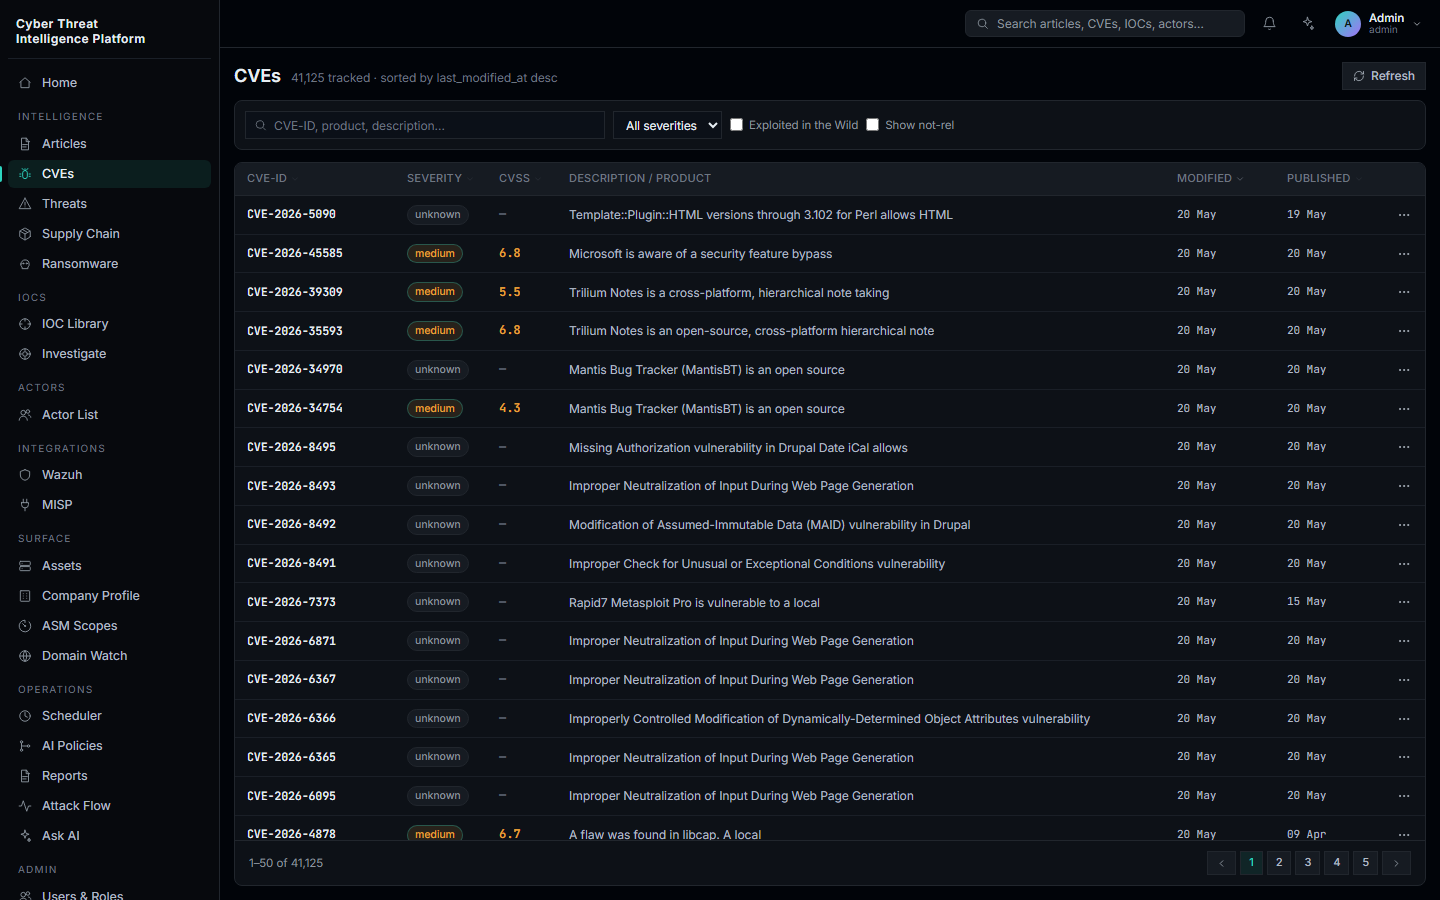
\includegraphics[width=0.88\textwidth]{images/tip/shots/06_cves_list.png}
\caption{Vulnerability-list workflow.}
\label{fig:cves-list-workflow}
\end{figure}

\begin{figure}[H]
\centering
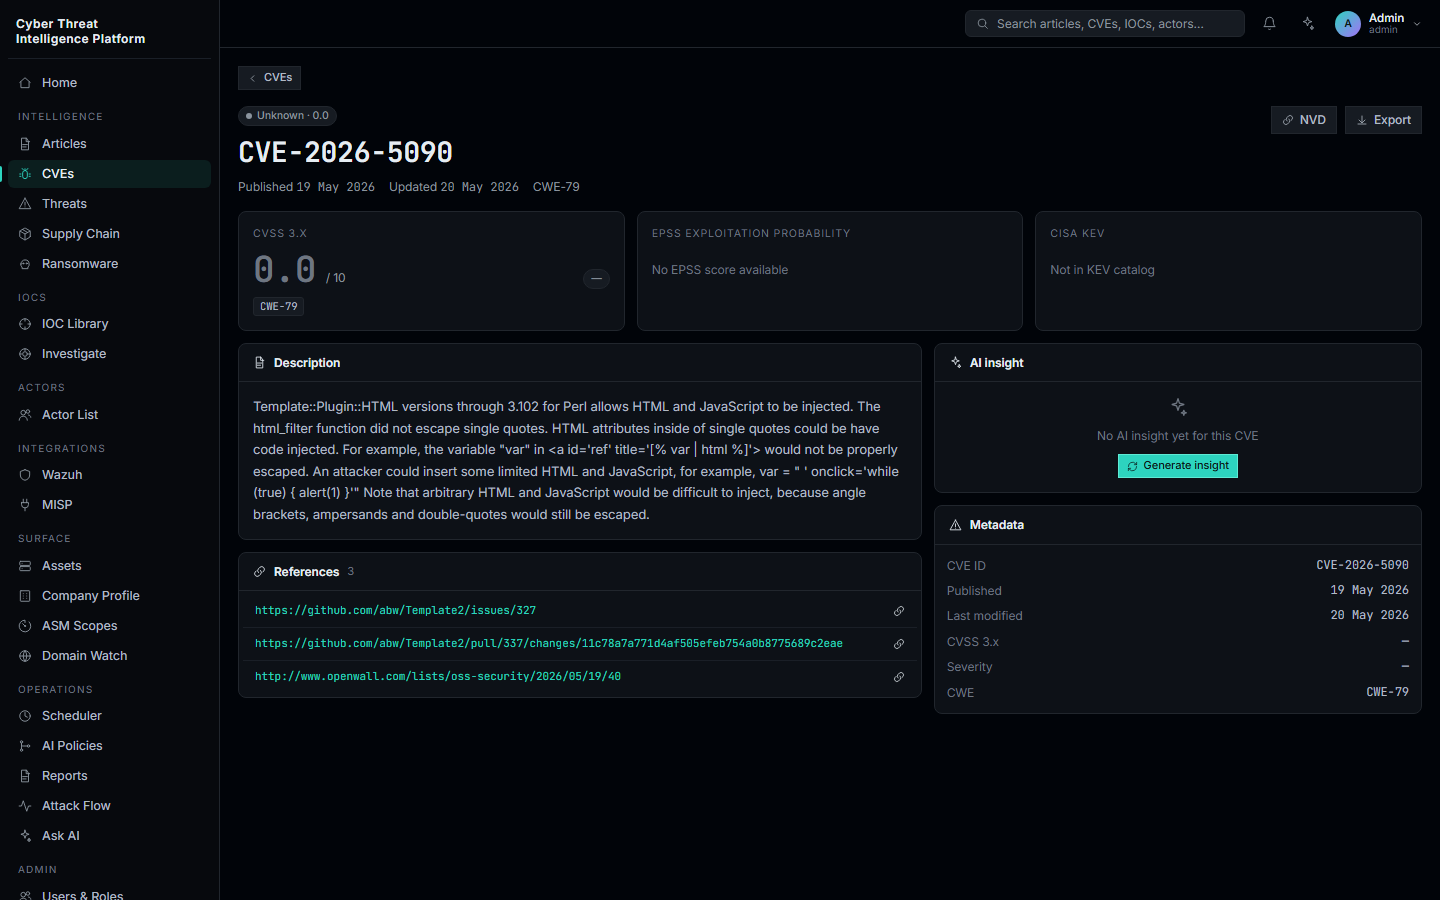
\includegraphics[width=0.88\textwidth]{images/tip/shots/07_cve_detail.png}
\caption{Vulnerability-detail workflow.}
\label{fig:cve-detail-workflow}
\end{figure}

\subsection{Threat and Actor Exploration}
Threat exploration workflows support higher-level intelligence interpretation. Analysts can move from lists of threats or actors to profiles, TTP associations, and AI-generated analytical tabs.

\begin{figure}[H]
\centering
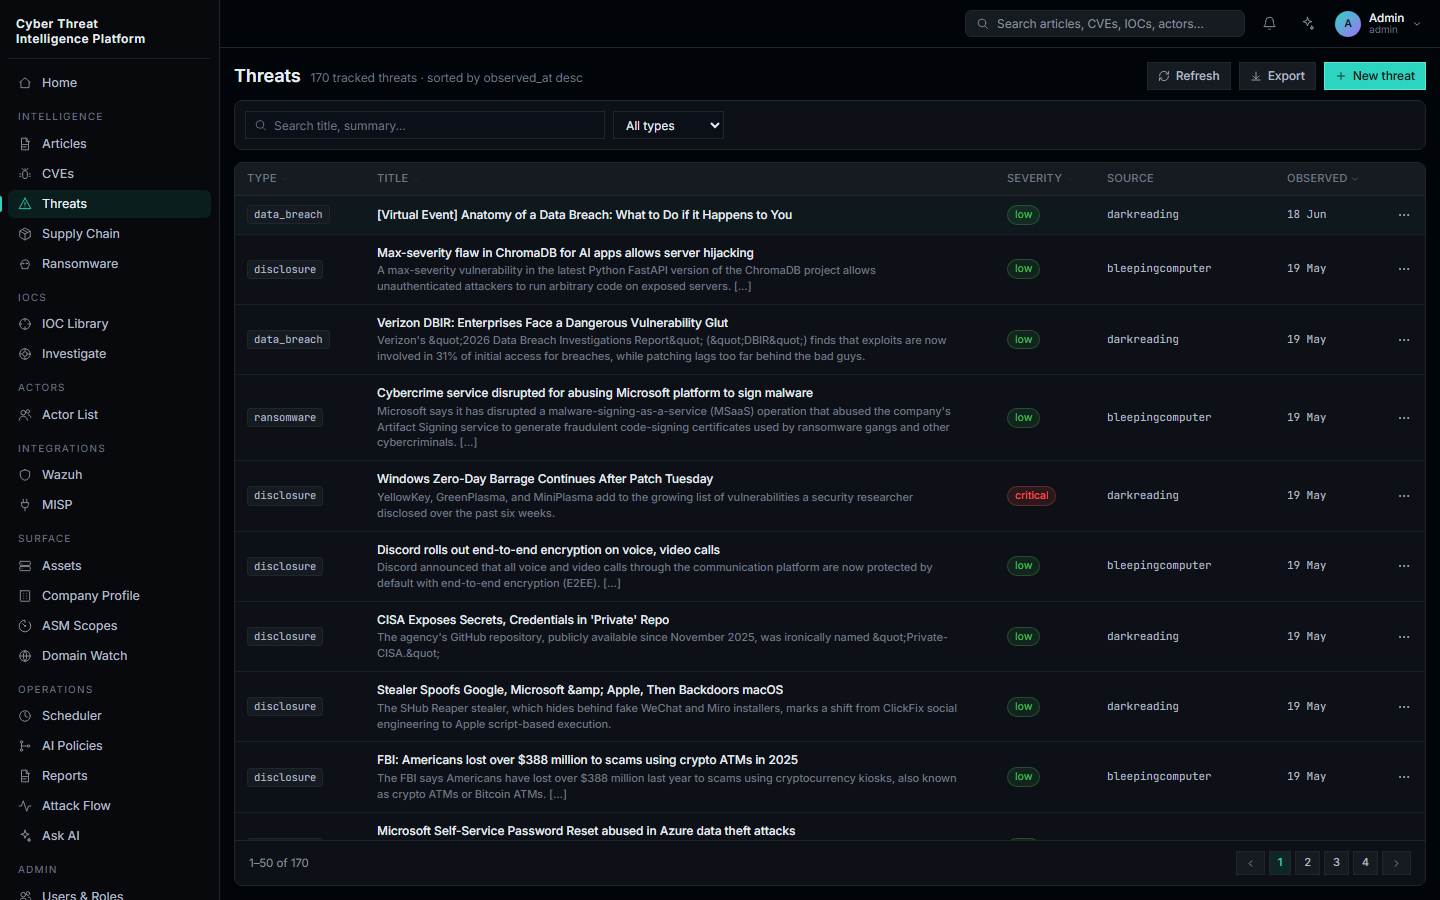
\includegraphics[width=0.88\textwidth]{images/tip/shots/08_threats_list.png}
\caption{Threat-list workflow.}
\label{fig:threat-list-workflow}
\end{figure}

\begin{figure}[H]
\centering
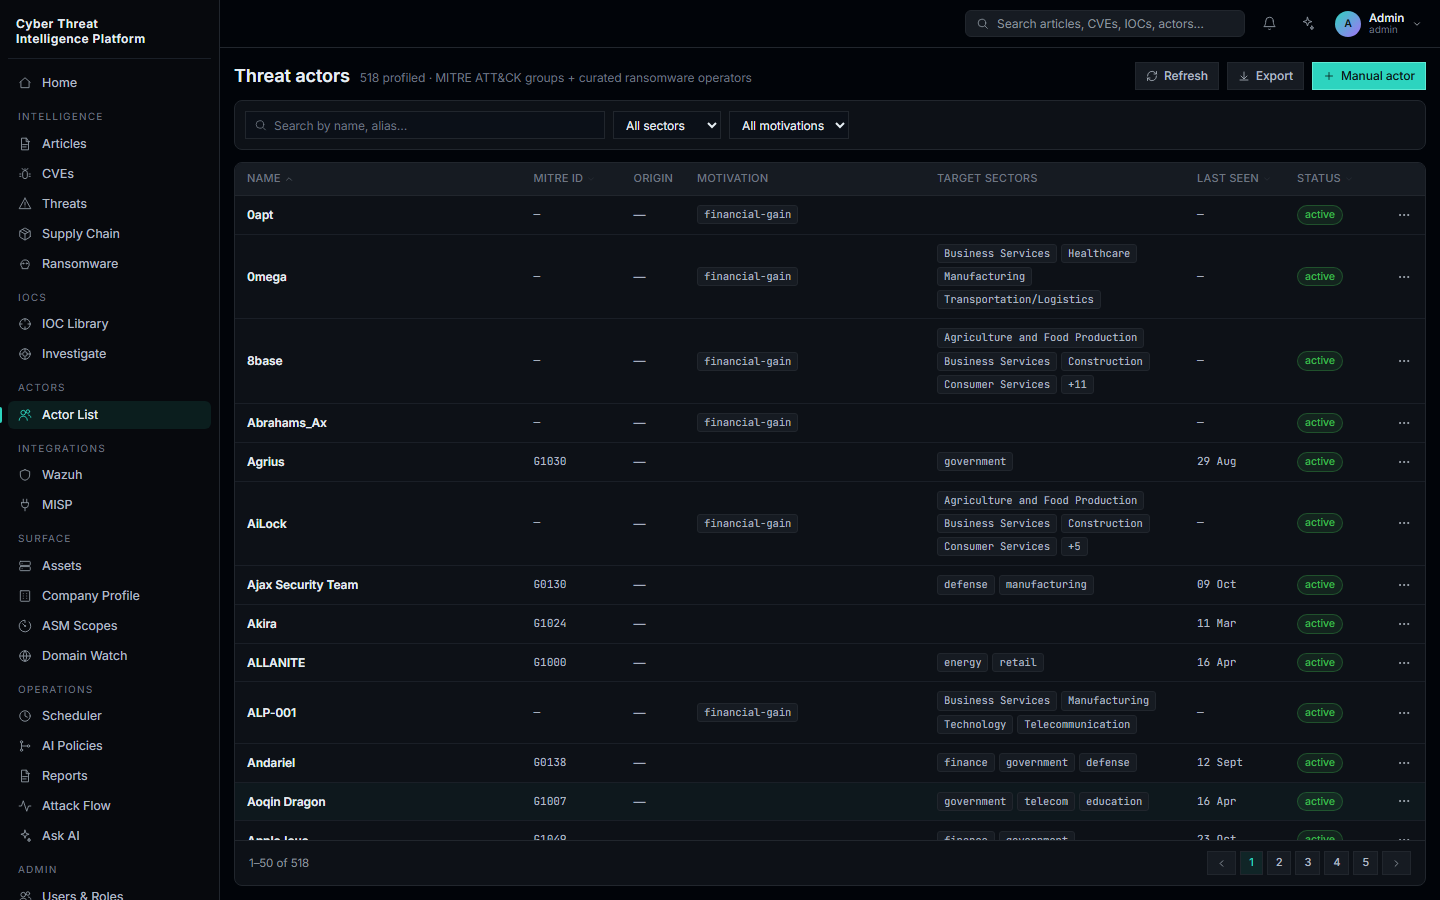
\includegraphics[width=0.88\textwidth]{images/tip/shots/18_actors_list.png}
\caption{Threat-actor list workflow.}
\label{fig:actors-list-workflow}
\end{figure}

\begin{figure}[H]
\centering
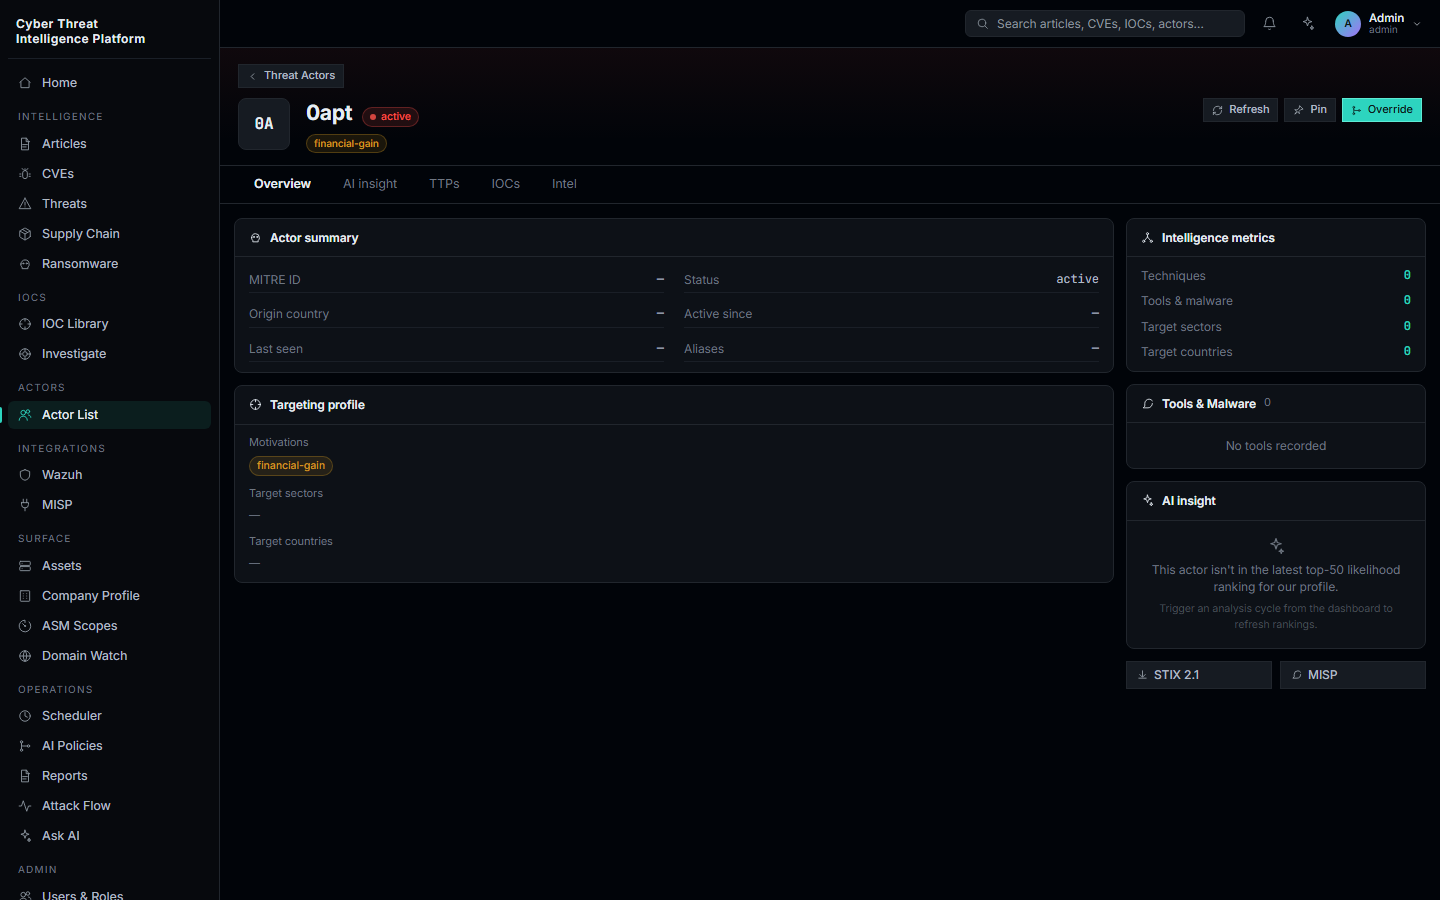
\includegraphics[width=0.88\textwidth]{images/tip/shots/19_actor_profile_overview.png}
\caption{Threat-actor profile workflow.}
\label{fig:actor-profile-workflow}
\end{figure}

\subsection{IOC Investigation Workflow}
The IOC workflow demonstrates the platform's dual-path design particularly well. The analyst can move from quick lookup to deeper investigation, with the latter using broader local and passive context.

\begin{figure}[H]
\centering
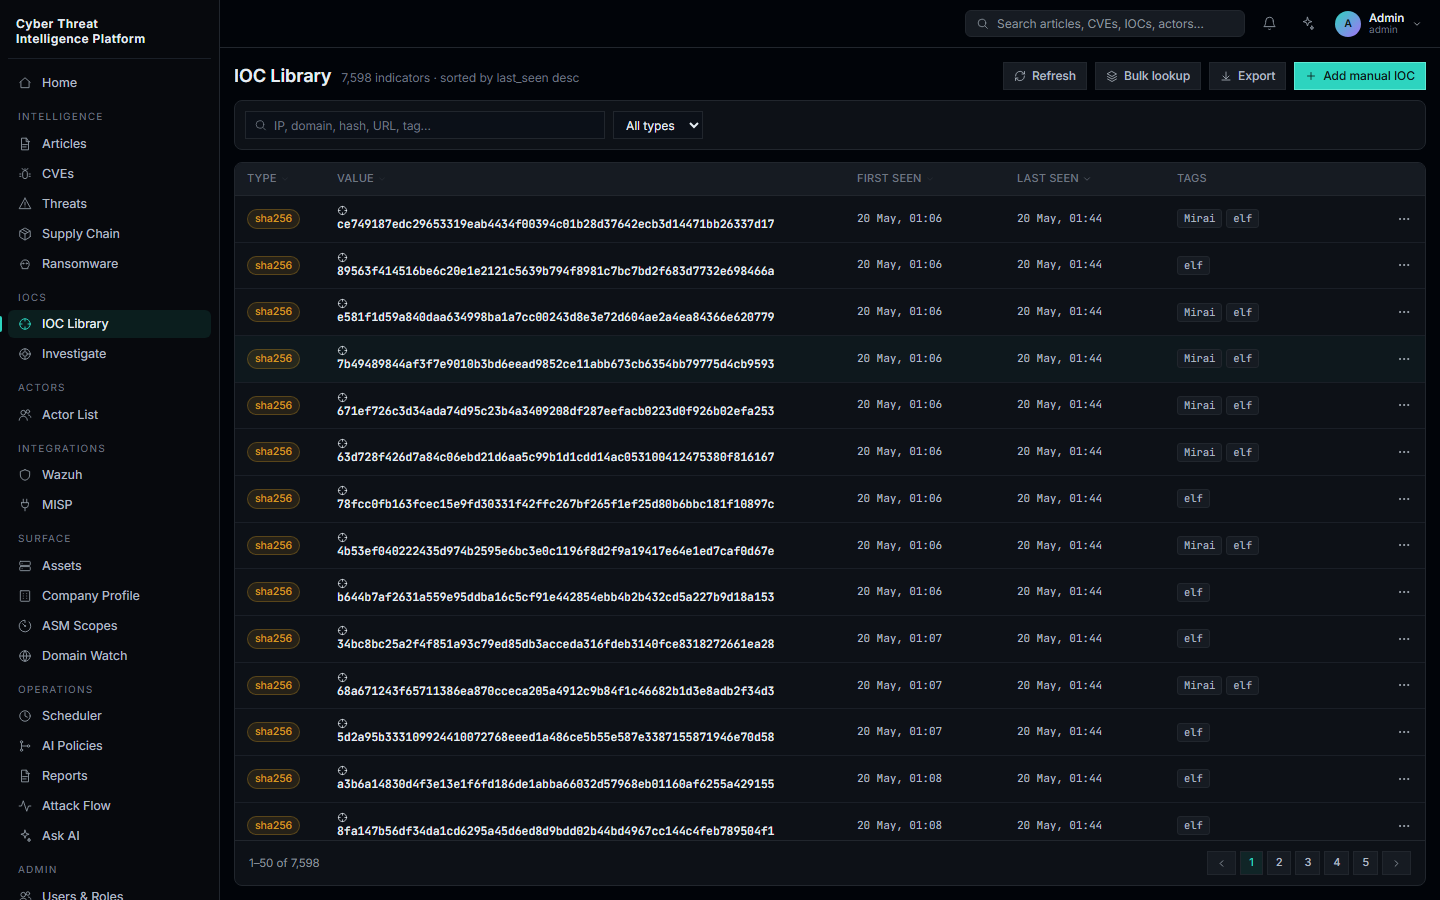
\includegraphics[width=0.88\textwidth]{images/tip/shots/13_iocs_library.png}
\caption{IOC-library workflow.}
\label{fig:ioc-library-workflow}
\end{figure}

\begin{figure}[H]
\centering
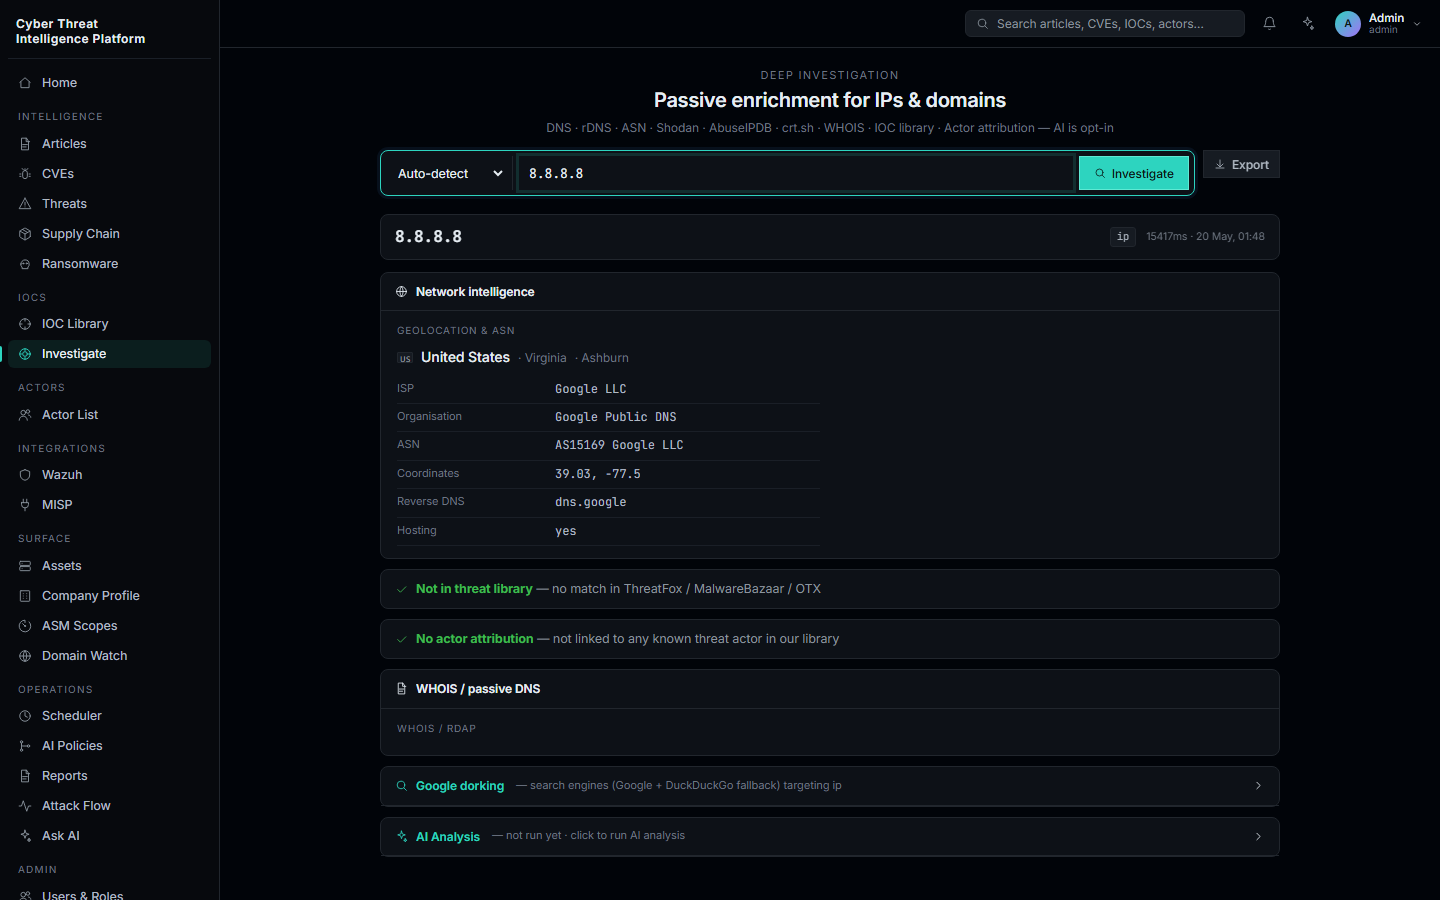
\includegraphics[width=0.88\textwidth]{images/tip/shots/16_ioc_investigate_result.png}
\caption{Deep IOC-investigation workflow.}
\label{fig:ioc-investigation-workflow}
\end{figure}

\subsection{Asset and Organization Context Workflow}
The asset and company-profile workflow is what allows the platform to move beyond generic feed consumption. It gives the system a local referent: which technologies, profiles, and exposures are actually relevant to the organization.

\begin{figure}[H]
\centering
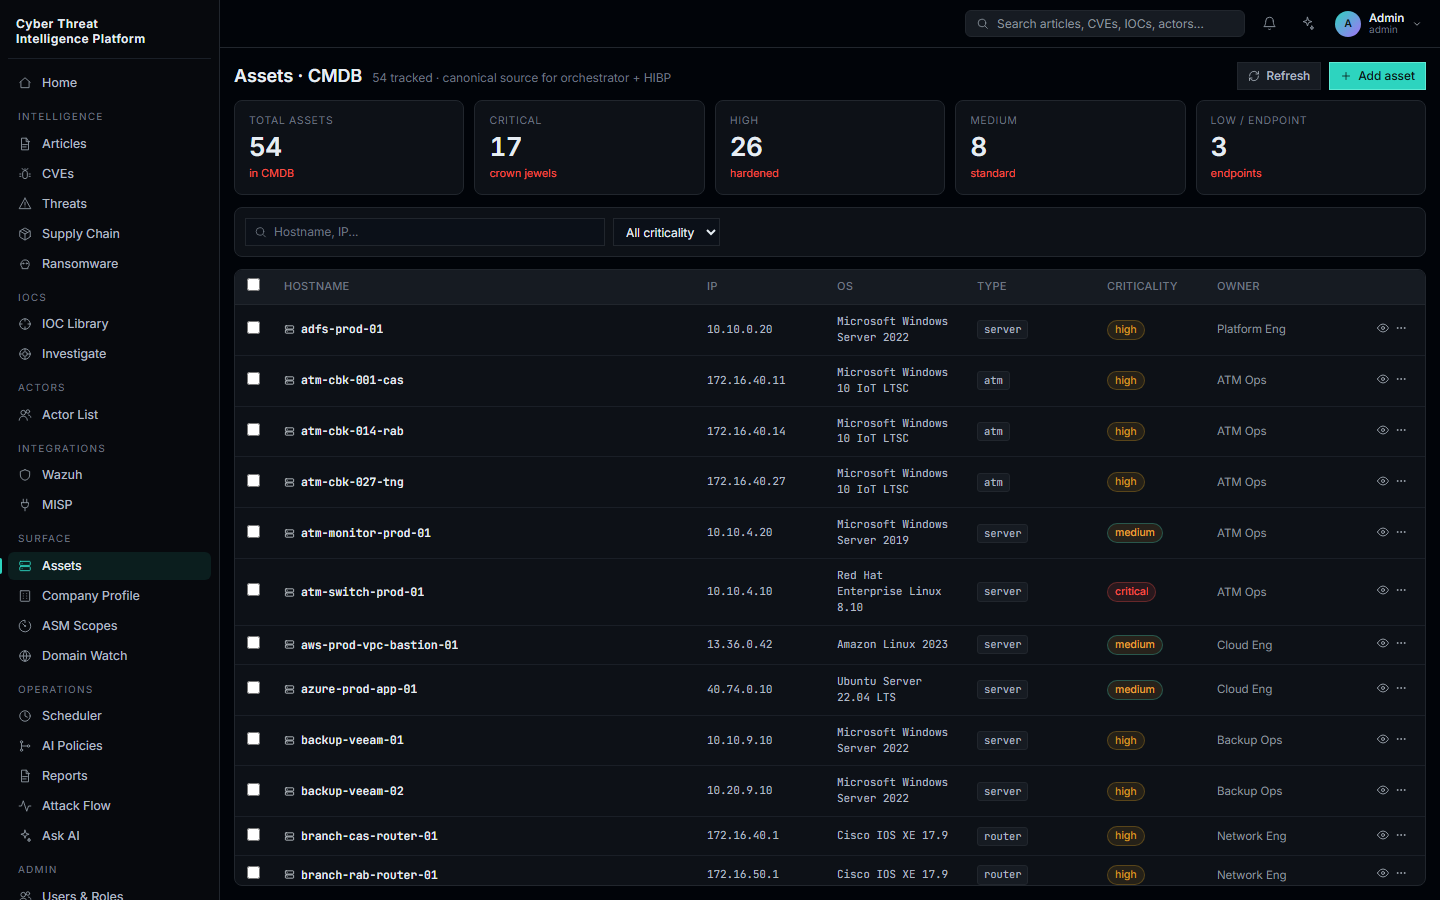
\includegraphics[width=0.88\textwidth]{images/tip/shots/22_assets_list.png}
\caption{Asset-list workflow.}
\label{fig:assets-list-workflow}
\end{figure}

\begin{figure}[H]
\centering
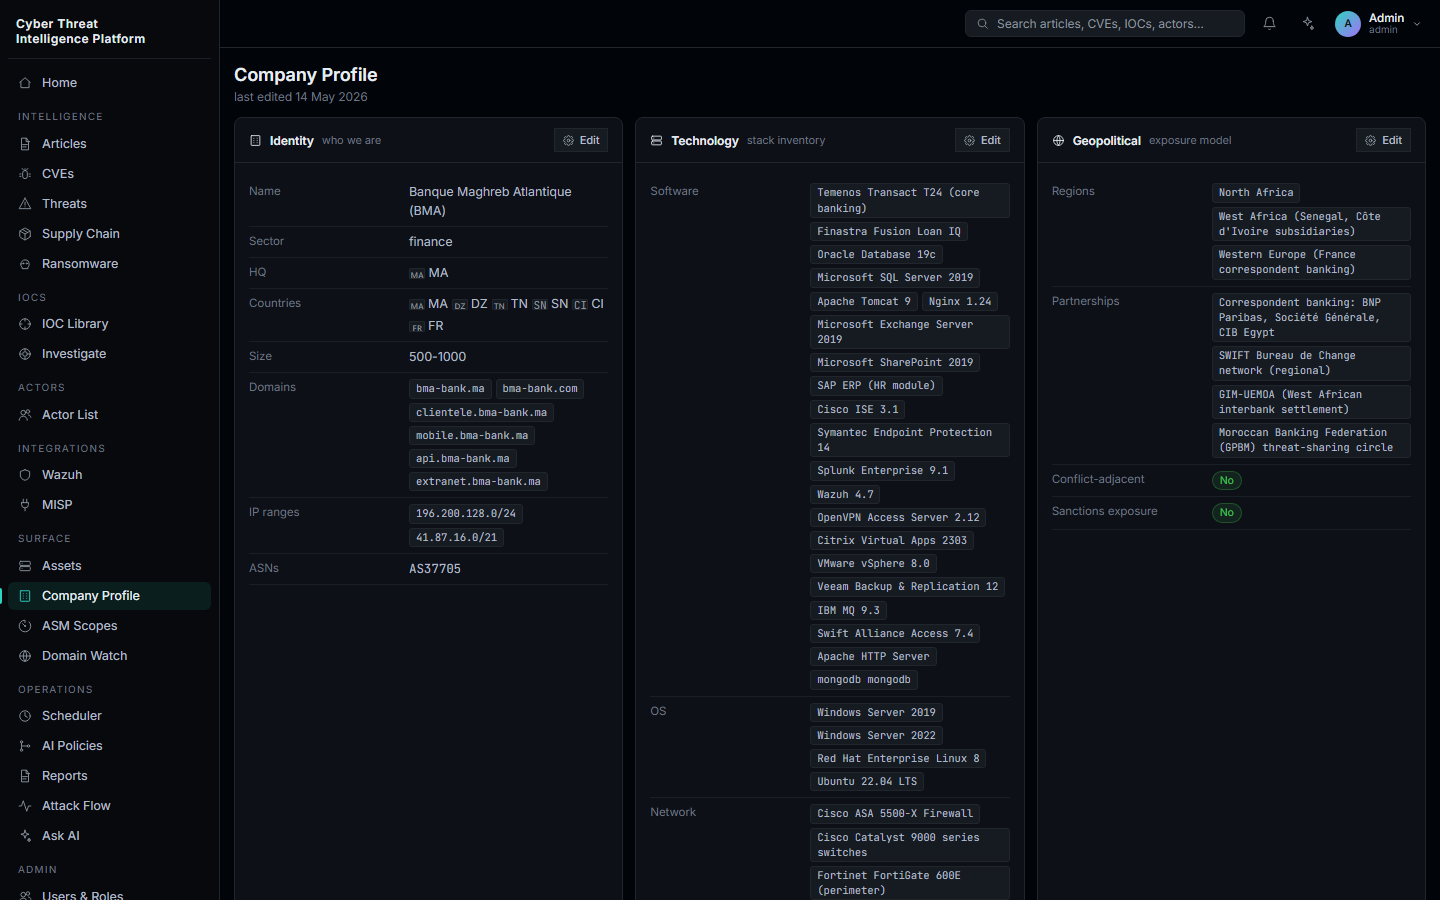
\includegraphics[width=0.88\textwidth]{images/tip/shots/23_assets_company_profile.png}
\caption{Company-profile workflow.}
\label{fig:company-profile-workflow}
\end{figure}

\subsection{Reports, Policies, and Administrative Workflows}
The reports, AI policies, settings, and administration pages show that the platform is not just an analyst sandbox. It is also a managed operational system with governance surfaces.

\begin{figure}[H]
\centering
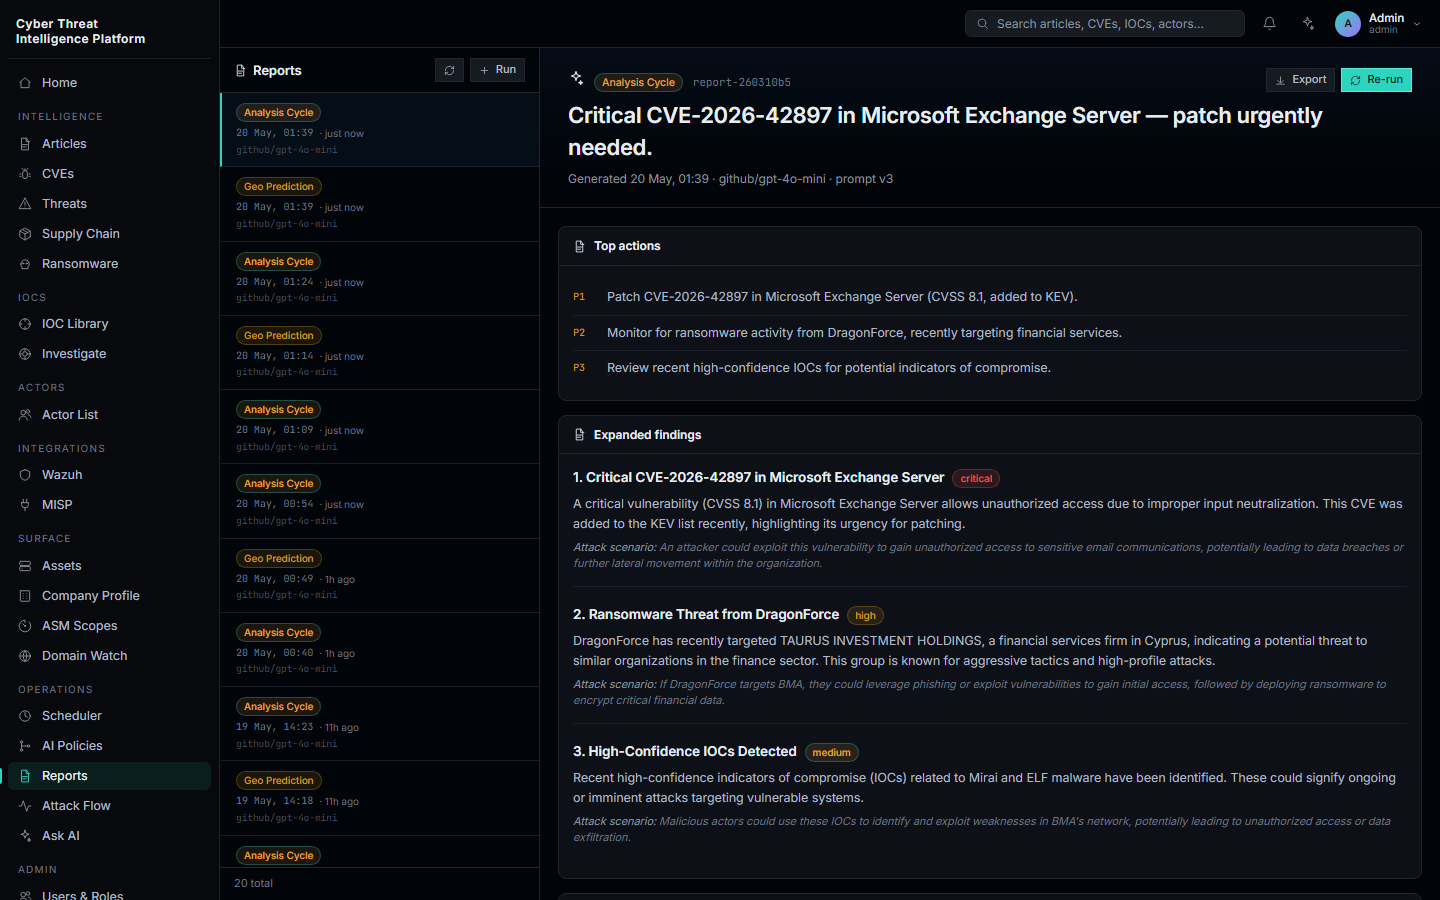
\includegraphics[width=0.88\textwidth]{images/tip/shots/31_reports.png}
\caption{Reports workflow.}
\label{fig:reports-workflow}
\end{figure}

\begin{figure}[H]
\centering
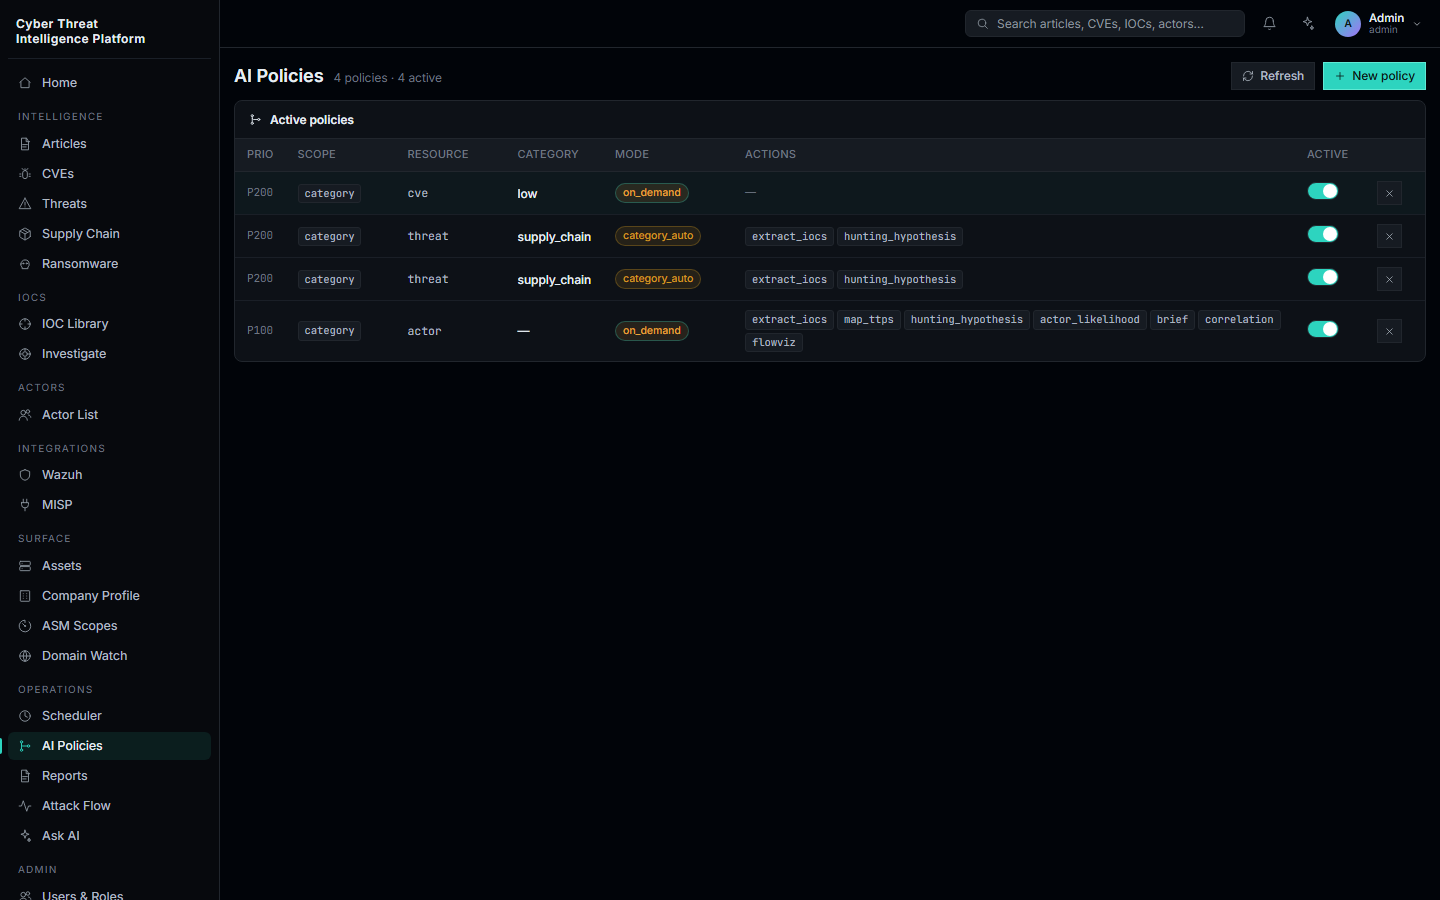
\includegraphics[width=0.88\textwidth]{images/tip/shots/30_ai_policies.png}
\caption{AI-policy workflow.}
\label{fig:ai-policy-workflow}
\end{figure}

\begin{figure}[H]
\centering
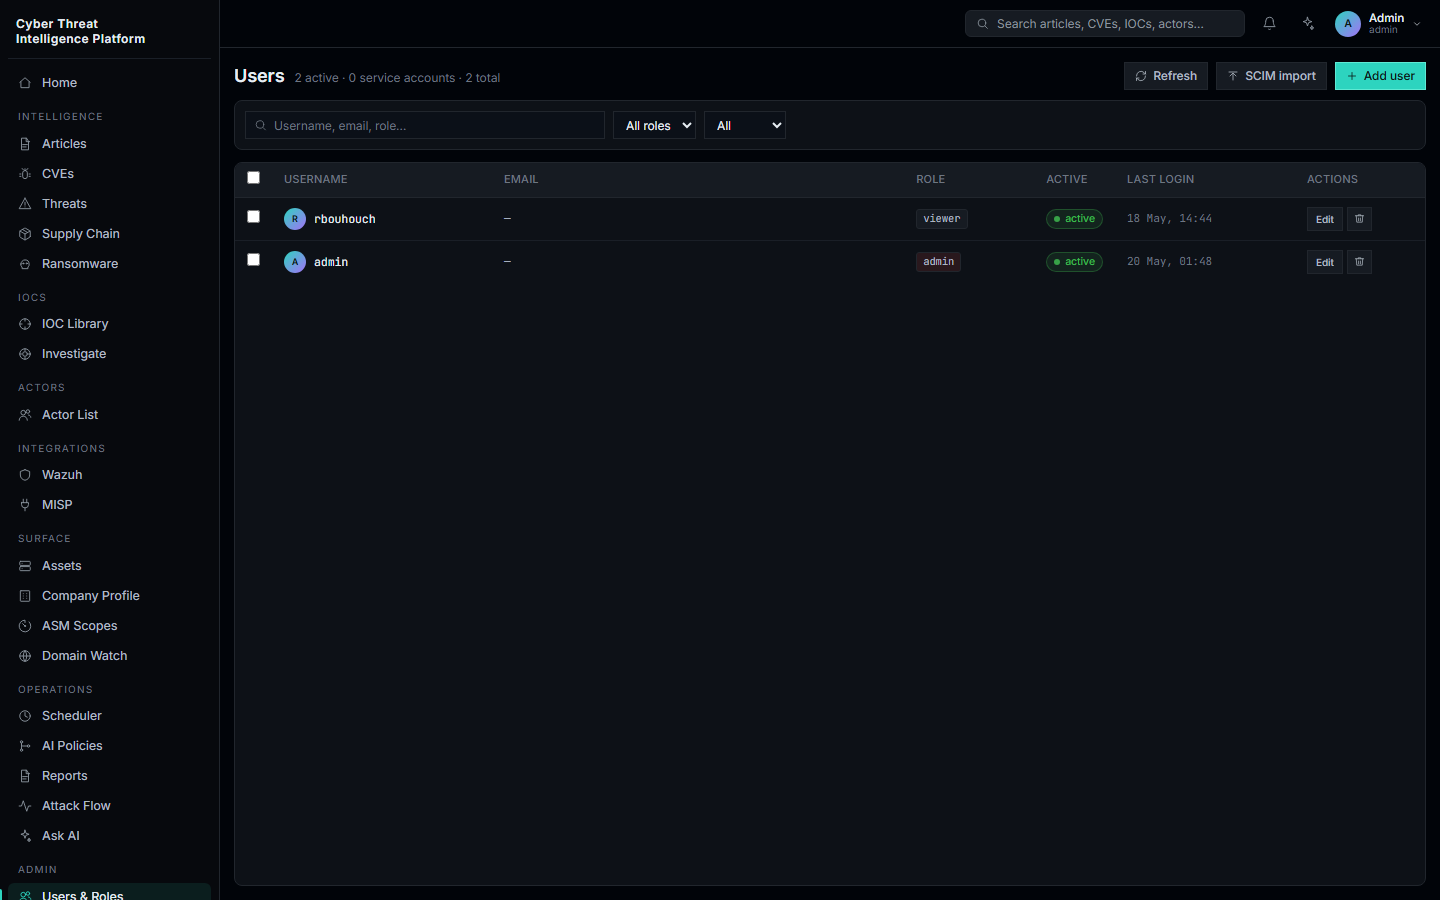
\includegraphics[width=0.88\textwidth]{images/tip/shots/34_admin_users.png}
\caption{Administrative user-management workflow.}
\label{fig:admin-users-workflow}
\end{figure}

\section{Why the Frontend Matters Architecturally}
It is tempting to treat the frontend as presentation only and therefore secondary in an architecture chapter. That would be a mistake here. The frontend determines how quickly analysts can convert platform capability into operational action. It also hosts the BFF, which means it participates directly in routing, aggregation, and edge trust. In this system, the frontend is therefore part of the architecture, not merely a decorative layer over it.

\section*{Conclusion}
\addcontentsline{toc}{section}{Conclusion}
The platform's data model, API design, and frontend workflows form one coherent chain. The data model defines what can be stored and correlated. The API layer defines how that knowledge is exposed and governed. The frontend defines how analysts and managers actually consume and act on the result. Understanding all three is necessary to understand why the platform works as an operational tool rather than only as a backend service collection.
